\documentclass[aip, jcp, reprint, twocolumn]{revtex4-2}

\bibliographystyle{apsrev4-2}

\usepackage{physics}
\usepackage{amsmath}
\usepackage{amssymb}
\usepackage{mathtools}
\usepackage{graphicx}
\usepackage{dcolumn}
\usepackage[colorlinks=true, linkcolor=black, urlcolor=blue, citecolor=black, anchorcolor=black]{hyperref}

\graphicspath{{"figures/"}}
\begin{document}
%Title of paper
\title{Coherent Hyper-Raman Four Wave Mixing Vibrational Spectroscopies}


\author{Ryan P. McDonnell} 
\author{Daniel D. Kohler}
\author{John C. Wright} \email{wright@chem.wisc.edu}

\affiliation{Department of Chemistry, 
        University of Wisconsin - Madison, 
        Madison, Wisconsin 53706, 
        United States of America}

\date{\today}

\begin{abstract}
Nonlinear, four wave mixing vibrational spectroscopies are often used to probe intramolecular vibrational coupling and relaxation dynamics.
Three wave mixing vibrational spectroscopies are similarly used to understand the spectroscopy and dynamics of interfacial species.
Most of these methods rely on infrared or Raman transitions to generate output. 
The implementation of a nonlinear hyper-Raman spectroscopy, which first appears at third order perturbation theory, can provide a useful analogue to these techniques to understand the spectroscopy and dynamics of isotropic systems.
Singly Vibrationally Enhanced (SIVE) spectroscopy, a type of nonlinear hyper-Raman spectroscopy, is an underdeveloped four wave mixing technique which shows promise as a method to disentangle ultrafast vibrational dynamics in isotropic systems without need for anharmonicities.
%alternate name is hyper-(S/D)FG... which is more interesting and descriptive than SIVE imo. lmk your thoughts
We derive selection rules for singly resonant SIVE (SR-SIVE) and demonstrate that SR-SIVE response extracts hyper-Raman polarizabilities ($\beta$).
The SIVE output is shown to be slightly stronger than vibrational sum frequency generation (vSFG), heavily driven by the number density probed by each process. 
The theory of SIVE is extended to account for vibronic coupling induced by two-photon absorption, i.e. doubly resonant SIVE (DR-SIVE), akin to resonant hyper-Raman spectroscopy. 
DR-SIVE is shown to be a type of resonance IR spectroscopy and is likely able to resolve vibronic coupling.
\end{abstract}

\maketitle

\section{Introduction}
Coherent multidimensional spectroscopy (CMDS) is a family of three and four wave mixing methods which form the optical analogue of multidimensional nuclear magnetic resonance (NMR) spectroscopy.\cite{Cho2008, RN335}
Multiresonant, four wave mixing CMDS experiments, first proposed by Oudar and Shen in 1980,\cite{RN307} directly probe coupling between different vibrational, electronic, and vibronic states. \cite{RN307, RN281, RN342, Cho2008, RN335, Ogilvie2019, RN325} 
CMDS has resolved anharmonicities and other intramolecular couplings in numerous systems. \cite{RN345, RN342, RN343, RN324, RN329, RN120, Czech2015, Gaynor2017, Ogilvie2019, RN325}
A particular class of CMDS methods, coherent Raman based four wave mixing spectroscopies, can provide explicit probes of vibrational and excitonic coupling in a variety of systems.

Not all CMDS methods are used to dissect intramolecular couplings.\cite{Shen1987_CPL}
Singly vibrationally enhanced (SIVE) is a four wave mixing method which, when detuned from  electronic resonances, does not probe intramolecular couplings. 
Non-parametric, singly resonant SIVE (SR-SIVE) spectroscopy was the first infrared CMDS method to successfully discriminate against non-resonant background.\cite{RN351, RN352}
In SR-SIVE, an infrared pulse is resonant with a vibrational mode, and two other input pulses are used to induce a scattering process to provide output.
SIVE was documented long ago to have characteristics similar to spontaneous hyper-Raman scattering spectroscopy. \cite{RN352}
Hyper-Raman scattering is the two photon analogue to Raman scattering. \cite{Cyvin1965, Terhune1965}
Compared to Raman spectroscopy, hyper-Raman scattering cross sections are often small, making it a difficult technique to successfully implement.\cite{RN515, Kelley2010} 
The different selection rules of hyper-Raman scattering, however, make it a unique alternative to Raman scattering to understand vibrational spectra and vibronic coupling in molecular systems.
In 1998, Cho et al. proposed a parametric six wave mixing technique which was the coherent analogue of hyper-Raman scattering. \cite{Cho1998}
However, since most six wave mixing methods cascade into four wave mixing processes,\cite{RN243, Cho2000_Cascade} it is preferable to investigate coherent four wave mixing analogues to hyper-Raman scattering.

While SIVE showed promise as an upconverted infrared spectroscopy method, it was quickly supplemented by a doubly vibrationally resonant method, doubly vibrationally enhanced (DOVE) spectroscopy, to investigate intra- and intermolecular vibrational coupling. \cite{RN345, RN101, Cho2000}
As a result, investigations of SIVE stagnated; to date, there are less than a dozen studies which report on SR-SIVE. \cite{RN350, RN416, RN351, RN352, RN353, Chen1998, RN362, RN418, Bonn2024, McDonnell2024}
Recent reports highlight non-negligible SIVE interference in DOVE experiments as well as the suitability of SIVE pathways to interpret ultrafast relaxation dynamics in isotropic systems. \cite{Bonn2024, McDonnell2024}
These reports motivate deeper analysis on the properties of SIVE spectroscopy. 

Fully coherent, ultrafast probes of vibronic coupling would yield insight into processes that control ultrafast electronic relaxation in molecular and biological systems. \cite{Bredenbeck2015, Arsenault2021}
Some years ago, Cho proposed a parametric, doubly resonant infrared/visible pathway to probe vibronic coupling in isotropic systems. \cite{Cho2001}
In this method, a single infrared pulse is resonant with a vibrational mode, and a two photon absorption event from a near infrared (NIR) or visible pulse resonant with an electronic or vibronic state is used to generate the four wave mixing signal.
These pathways are referred to herein as DR-SIVE.
Methods analogous to DR-SIVE, where two photon absorption from the infrared pulse and single photon absorption from the visible pulse is used to generate output, i.e., stimulated Raman processes, have been reported. \cite{RN301, RN120} 

An experimental complexity in executing four wave mixing experiments is the demand of three separate input pulses, often all at different frequencies.
For example, in the case of DOVE, two of the three input pulses must be scanable infrared pulses. \cite{RN345} 
Only recently have methods been developed for seamless tuning and scanning of ultrafast optical parametric amplifiers across swaths of frequency space. \cite{RN162, McDonnell2024, SkyeOPA, KyleOPA}
Since SR-SIVE demands only a single resonance to be scanned, the experiment can be performed using two input pulses: one tunable, infrared OPA to scan across vibrational resonances, and a two photon absorption from the signal process of a separate OPA, or output from the oscillator which pumps the infrared OPA.
As such, laboratories experienced in sum frequency generation (SFG) spectroscopy can perform SIVE spectroscopy to understand bulk dynamics and spectroscopy using nearly the same setup.\cite{Shen1987_CPL}

Inspired by recent work which demonstrated the presence of SIVE in ultrafast DOVE experiments,\cite{McDonnell2024} we investigate the parameters which result in both SR and DR-SIVE output. \cite{Cho2000, Bonn2024}
We develop simple expressions which relate transition dipoles and hyper-Raman polarizabilties and the overall SR-SIVE output, yielding gross selection rules. 
It is shown that a SIVE active mode must be both IR and hyper-Raman active.
Since any IR active vibration is also hyper-Raman active, \cite{Andrews1978} we demonstrate that SIVE is a coherent analogue of hyper-Raman scattering spectroscopy for IR active vibrations, i.e., SIVE is an optically upconverted infrared spectroscopy.
This is akin to sum and difference frequency generation (SFG, DFG) being coherent Raman analogues for IR active vibrations. \cite{Shen90}

We investigate properties of doubly resonant SIVE (DR-SIVE) to understand how coupling between vibrational and vibronic states can be measured through DR-SIVE.
DR-SIVE is shown to demand one and two-photon absorptions between the ground and excited state.
DR-SIVE is thus the four wave mixing analogue of doubly resonant infrared-visible sum frequency generation. \cite{Shen94}

\section{Results and Discussion}
Singly resonant SIVE (SR-SIVE) spectroscopy has potential to provide deeper insight into single quantum decoherence times and molecular orientation in condensed systems.
Similarities between SR-SIVE spectroscopy, infrared spectroscopy and spontaneous hyper-Raman scattering have been noted previously. \cite{RN352, Bonn2024}
In this section, we make the connections between SIVE and hyper-Raman scattering explicit and remark on the properties of SIVE that become apparent after inspecting the selection rules.

\begin{figure}[!htbp]
	\centering
	\includegraphics[width=3.375in]{wmel1.png}
	\caption{Wave Mixing Energy Level (WMEL) diagrams of the relevant SR-SIVE pathways in the (a) $\vec{k}_4 = -\vec{k}_1 + \vec{k}_2 + \vec{k}_3$ and (b) $\vec{k}_4 = \vec{k}_1 + \vec{k}_2 + \vec{k}_3$ phasematching geometries. \cite{RN286, RN352}
	$\ket{g}$ is the ground state, $\ket{v}$ is an infrared active vibration and $\ket{m}, \ket{n}$ are virtual states.
	Solid and dashed horizontal lines indicate real and virtual states, whereas solid and dotted arrows indicate ket and bra side transitions, respectively. 
	These diagrams can be permuted to generate additional resonant WMEL diagrams.}
	\label{fig:sivewmel}
\end{figure}

It is useful to expose relationships between transition dipoles, Raman polarizabilities and hyper-Raman polarizabilities in the driven limit. \cite{Simpson2004, RN120}
In the driven limit, under the electric dipole approximation, the I$^{th}$ component of the third order nonlinear output polarization, ${P}^{(3)}_I$, of any four wave mixing process, induced by electric fields E, at output frequency $\omega_4$ is written as \cite{RN307}
\begin{equation} \label{polarization}
{P}^{(3)}_I (\omega_4)  = \chi^{(3)}_{IJKL} E_J E_K E_L 
\end{equation}
where $\chi^{(3)}_{IJKL}$ is the IJKL element of the third order electrical susceptibility, a rank four tensor, generally written as
\begin{equation}
	\chi^{(3)}_{IJKL} = NF(\omega_4) \langle \gamma_{ijkl} \rangle
\end{equation}
where N is a number density, F is the Lorentz local field factor, and $\gamma_{ijkl}$ is the third order polarizability (i.e., second hyperpolarizability). 
The brackets indicate an orientational average. 
Uppercase letters refer to laboratory frame coordinates and lower case letters refer to molecular frame coordinates.

\subsection{Vibrational SR-SIVE Selection Rules}
To make the connection between SR-SIVE and hyper-Raman scattering, we investigate the gross selection rules of SR-SIVE-IR.
By propagating density matrix elements in the steady state limit, the SIVE hyperpolarizability is \cite{RN119}
\begin{equation}\label{sivegamma}
		\gamma_{ijkl} =	- \sum_{m, n} \frac{1}{\varepsilon_0} \frac{1}{4D} \frac{1}{\hbar^3} \frac{\mu^{i}_{v n} \mu^{j}_{nm} \mu^{k}_{mg} \mu^{l}_{gv} }{\Delta_{nv} \Delta_{mv}\Delta_{gv}}  \rho_{gg}
\end{equation}
where: $\mu^{j}_{ab}$ is the $j^{th}$ element of $\mel{a}{\vec{\mu}}{b}$, $\Delta_{kl} = \omega_{kl} - \omega_{j} - i\Gamma_{kl}$, $\omega_j$ is the frequency of the j$^{th}$ input field, $\Gamma_{kl}$ is the dephasing of $\rho_{kl}$ and $\rho_{gg}$ is the ground state population.
For simplicity, we consider the results for the process diagrammed in \autoref{fig:sivewmel}a, but by multiplying by (-1) and taking a complex conjugate, which arise from the bra-side transition in \autoref{fig:sivewmel}a, results for the \autoref{fig:sivewmel}b  process are obtained.
Note that $\omega_j \rightarrow -\omega_j$ for a bra side transition.
D, the Maker-Terhune degeneracy factor, accounts for permutation symmetry in $\gamma_{ijkl}$ and is defined as $\frac{n!}{(n-m)!}$, where $n$ is the total number of input fields (3 for any four wave mixing experiment) and $m$ is the number of distinguishable input fields.\cite{RN134} 
For a SIVE experiment using two or three distinct input fields, as considered here, D = 6.
Note that $\ket{m}, \ket{n}$ are virtual states (\autoref{fig:sivewmel}).
By contracting over the virtual states to form the hyper-Raman hyperpolarizability $\beta$ (i.e., Placzek approximation), this expression can be simplified immensely.\cite{Long1970} 
Note, however, that if $\omega_2$, $\omega_3$, as depicted in \autoref{fig:sivewmel}, are nearly resonant with any state, the Placzek approximation fails. \cite{Placzek1934, Long1970}
Assuming the validity of the Placzek approximation, \autoref{sivegamma} is written as 
\begin{equation}\label{sivebeta}
	\gamma_{ijkl} =	-\frac{1}{\varepsilon_0} \frac{1}{24 \hbar}\frac{\beta^{(ijk)}_{gv} \mu^{(l)}_{gv}}{\Delta_{gv}} \rho_{gg}
\end{equation}
As such, any mode that is SIVE active must be both hyper-Raman and IR active.
However, since any IR active vibrational mode is hyper-Raman active,\cite{Cyvin1965, Andrews1978} any IR active mode is SIVE active.
This makes SIVE an optically upconverted infrared spectroscopy of isotropic samples, as its selection rules are identically those of IR spectroscopy, but its output is generally in the visible.
Unlike SFG spectroscopy, which is dependent upon both the infrared and Raman activity of a mode (through symmetry constraints, this demands that the microscopic SFG output from centrosymmetric species vanishes),\cite{Shen90, Cotton} SIVE is a nonlinear, optically upconverted spectroscopy for any infrared active mode.

To understand SR-SIVE selection rules more finely, the dipole and first hyperpolarizability operators are Taylor expanded in terms of an n$^{\text{th}}$ normal mode coordinate $Q_n$ about equilibrium: \cite{Long1970}
\begin{subequations}
	\begin{equation}
		\mu = \mu_0 + \frac{\partial \mu}{\partial Q_n} Q_n + \order{{Q_m Q_n}}
	\end{equation}
	\begin{equation}
		\beta = \beta_{0} + \frac{\partial \beta}{\partial Q_n} Q_n + \order{{Q_m Q_n}}
	\end{equation}
\end{subequations}
Substituting into \autoref{sivebeta}, and knowing that $\mel{v}{Q_n}{g} = \sqrt{\frac{\hbar}{2m_n\omega_{vg}}}$ under the harmonic approximation,\cite{RN230} where $m_n$ is the mass of the $Q_n$ mode, gives the SIVE-IR-I hyperpolarizability to $\order{Q_n}$ as \begin{equation}\label{SIVEselection}
		\gamma_{ijkl} =	-\frac{1}{\varepsilon_0} \frac{1}{48 m_n \omega_{vg}}  \frac{1}{{\Delta_{gv}}} \ \frac{\partial \beta^{(ijk)}}{\partial Q_n} {\frac{\partial \mu^{(l)}}{\partial Q_n}}  \rho_{gg}
\end{equation}
Since this expression is non-zero in the harmonic oscillator limit, SR-SIVE output is allowed for harmonic transitions. 
Similar to SFG, SR-SIVE does not demand anharmonic ground state potential energy surfaces for spectral output. \cite{Shen94, Cho2000}
This selection rule is generally valid for any SR-SIVE process in the $-\vec{k}_1 + \vec{k}_2  + \vec{k}_3$ and $\vec{k}_1 + \vec{k}_2  + \vec{k}_3$ phasematching geometries when the Placzek approximation is valid.

A useful attribute of this selection rule is the added ability of polarization control arising from the hyperpolarizability tensor. 
Similar to polarization control in second harmonic and sum frequency generation experiments which probe different elements of the infrared transition dipole and Raman polarizability tensor,\cite{Heinz1982} probing different elements of the hyperpolarizability tensor in SR-SIVE can greatly assist in understanding ultrafast dynamics in isotropic systems. \cite{Shen90, Bonn2024}
Polarization control in IR-pump-SIVE-probe, analogous to ultrafast transient absorption spectroscopy, would be an interesting venue to assess the sensitivity of SR-SIVE to different hyper-Raman tensor elements.

\subsection{Comparison to Sum Frequency Generation}
Since the hyper-Raman process is effectively a two-photon process, a setup using only two lasers can perform the SIVE experiment by investigating $\pm \vec{k}_1 + 2\vec{k}_2$ processes.
The other commonly used two laser CMDS method is sum frequency generation, a $\chi^{(2)}$ technique, whose phasematching is dictated by $\vec{k}_1 + \vec{k}_2$.
The SFG output scales as $\chi^{(2)}_{IJK} \sim \langle \alpha_{ij} \mu_k \rangle$, where $\alpha_{ij}$ is the Raman polarizability tensor.
Since SFG is dependent upon transitions that transform like both rank-one and rank-two tensors, this enforces a microscopic constraint that SFG cannot yield output for centrosymmetric species under the electric dipole moment.
This follows from simple parity arguments, where inversion centers demand states possess distinct parity selection rules. \cite{RN230}
Macroscopically, inversion symmetry in the output polarization eliminates output from centrosymmetric species under the electric dipole approximation.
As a result, the output of SFG is significantly reduced relative to most third order spectroscopies because the output only depends on surface species.
However, since SIVE spectroscopy is dependent upon a hyper-Raman transition, it is useful to compare the relative output of the two processes to identify how SIVE output compares to SFG.

To motivate the application of SIVE spectroscopy, we perform a calculation to compare the output of parametric SIVE-IR (\autoref{fig:sivewmel}b) to that of vibrational SFG (vSFG) spectroscopy.
Absorption effects are neglected for simplicity.
\begin{widetext}
To allow comparison between the two methods, the output polarizations of each process is written as
	\begin{subequations}
		\begin{equation}
			\abs{P^{(2)}_{\text{SFG}}} = N_{surf} F(\omega_1+\omega_2) \abs{\langle \alpha_{ij}\mu_{k} \rangle E_J(\omega_2)E_K(\omega_1)} 
		\end{equation}
		\begin{equation}
			\abs{P^{(3)}_{\text{SIVE}}} = N_{bulk}  F(\omega_1+\omega_2 +\omega_3) \abs{\langle \beta_{ijk} \mu_{l} \rangle E_J{(\omega_3)}E_K(\omega_2)E_L(\omega_1)} \ell_{eff}
		\end{equation}
	\end{subequations}
where N$_{bulk}$ is the bulk number density, and N$_{surf}$ is the surface number density (10$^{19}$ m$^{-2}$).\cite{RN133, RN503}	
For liquids with molar masses less than $\sim$100 g mol$^{-1}$ and densities roughly equal to that of H$_2$O$_{(l)}$ at room temperature, N$_{bulk} \sim$ 10$^{28}$ m$^{-3}$.
We take the bulk optical interaction length ($\ell_{eff}$) to be 10 $\mu$m.\cite{RN133} %see chapter 25 of Shen's NLO book... idk something here seems wrong
A normal dispersion curve is assumed so that $F(\omega_1+\omega_2) \approx F(\omega_1+\omega_2 +\omega_3)$.
To simplify analysis, orientational averaging is ignored (e.g., $\langle \beta_{ijk} \mu_{l} \rangle \approx \beta \mu$) and the input and output fields are taken to be co-polarized, so that
\begin{equation}
		P_{ratio} \equiv \frac{\abs{P^{(3)}_{\text{SIVE}}}}{\abs{P^{(2)}_{\text{SFG}}}} \approx \frac{N_{bulk}}{N_{surf}} \frac{\beta}{\alpha} E(\omega_3) \ell_{eff} \sim 10^4 \frac{\beta}{\alpha} E(\omega_3)\\
\end{equation}
\end{widetext}
Ziegler has noted that for a field of intensity 10 GW/cm$^{2}$, $\frac{\beta E}{\alpha} \sim 10^{-3} $ for vibrational modes when $E(\omega_3)$ is largely detuned from electronic resonances. \cite{RN515}
Such an intensity is easily obtained using modern ultrafast sources.
In this limit,
\begin{equation}
\begin{split}
		P_{ratio} &\sim 10^4 \frac{\beta E(\omega_3)}{\alpha} \sim 10
\end{split}
\end{equation}
Since the intensity ratio scales as $\abs{P_{ratio}}^2$, we see that the SIVE output is somewhat stronger than vibrational SFG, assuming only interfacial contributions in vSFG.
It is important to note that this derivation ignored absorption and orientational averaging effects, which can significantly reduce output from either process. 



\subsection{Quantitative SR-SIVE}
With the selection rules of SR-SIVE understood for vibrational spectroscopy, it becomes possible to extract quantitative information from SIVE spectra to compare to incoherent methods and other CMDS methods.
Lineshape analysis is essential for extracting quantitative information from CMDS spectra.
Scanning across resonances create dispersive lineshapes, i.e, self-heterodyning, which inform on $\Re(\chi^{(3)})$ and $\Im(\chi^{(3)})$.\cite{Levenson1974_1, Levenson1974_2}
In the method introduced by Levenson and Bloembergen (Bloembergen Interferometry Experiment), an internal standard interferes with the resonant lineshape.
The internal standard is often chosen to be C$_6$H$_6$ or C$_6$D$_6$, due to the strong Raman activity and measured $\chi^{(3)}$ of its ring breathing mode ($\nu_2$ in Herzberg notation). \cite{Levenson1974_2, RN351, RN345}
Self-heterodyning of the internal standard signal measures $\chi^{(3)}$ and does not require measurement of absolute intensities. 
Resonant lineshapes are also complicated by amplitude level interference between the sample and its substrate and/or sample cell windows, which must be accounted for to obtain quantitatively correct $\chi^{(3)}$ values. \cite{RN362, RN418}

Most quantitative methods in an n$^{th}$ order CMDS experiment are used to extract $\chi^{(n)}$ values to compare the relative strength of nonlinear processes in different media. \cite{Zhu87, RN351, RN345}
The recorded $\chi^{(n)}$ values provide insight into how microscopic quantities ($\vec{\mu}, \alpha_{ij}, \beta_{ijk}$) impact nonlinear output.
To our knowledge, only vibrational SFG and 2D-IR spectroscopy has taken advantage of orientationally averaged $\chi^{(n)}$ values to extract transition moments. \cite{Shen90, Moilanen2009, RN245}
Previous treatments did not consider using quantitative analysis in SIVE to measure $\beta_{ijk}$ values from SIVE spectra.
It is thus useful to investigate how a simple treatment of orientational averaging can extract $\beta_{ijk}$ from $\chi^{(3)}_{IJKL}$.

The SIVE $\chi^{(3)}_{IJKL}$ expression is
\begin{equation}\label{chi3}
\begin{split}
		\chi^{(3)}_{IJKL} &= NF(\omega_4) \langle \gamma_{ijkl} \rangle = -\frac{NF}{24 \hbar \varepsilon_0 \Delta_{gv}} \langle \beta_{ijk} \mu_l \rangle \rho_{gg}\\
\end{split}
\end{equation}
This expression cannot be used as written to extract $\beta_{ijk}$, as $\beta_{ijk}$ is a Hermitian operator, but $\Delta_{gv} \in \mathbb{C}$. 
However, since the real and imaginary parts of $\chi^{(3)}$ can be extracted from the Bloembergen interferometry experiment, we can choose to focus on either its real or imaginary part.
For simplicity, we investigate $\Im(\chi^{(3)})$, giving, assuming resonance conditions, 
\begin{equation}
	\langle \beta_{ijk} \mu_{l} \rangle = \frac{24 \hbar \varepsilon_0}{NF} \Gamma_{gv} \frac{1}{\rho_{gg}} \Im(\chi^{(3)}_{IJKL})
\end{equation}

The steps behind orientational averaging of $\gamma_{ijkl}$, a rank four tensor in the molecular frame, are detailed elsewhere.\cite{Andrews1977, McDonnell2024}
Orientational averaging shows specific polarization schemes isolate linear combinations of different $\beta_{ijk}$ terms. 
Infrared spectra can provide values for different $\vec{\mu}$ components.
Since $\vec{\mu}$ is a rank-one tensor, its three Cartesian components share the simple relationship $\langle {\mu^2_x} \rangle = \langle {\mu^2_y} \rangle = \langle {\mu^2_z} \rangle = \frac{1}{3}\langle {\mu^2} \rangle$. \cite{RN459}
Neglecting rotational dependence (i.e., assuming only vibrational transitions), $\langle {\mu^2} \rangle = \abs{\mu}^2 = \mu^2$, so that $\langle \beta_{ijk} \mu_l \rangle = \langle \beta_{ijk} \rangle \frac{\mu}{\sqrt{3}}$.
By introducing the reduced mass coordinate $q_n = \sqrt{\frac{1}{m_n}} Q_n$ and using the expansions of $\beta_{ijk}$ and $\mu_{l}$ to $\order{Q_n}$ found earlier, we see
\begin{equation}\label{betasive}
	\langle \frac{\partial \beta_{ijk}}{\partial q_n} \rangle = \varepsilon_0 \frac{48 \sqrt{3} }{NF}  \frac{\Gamma_{gv} \omega_{vg}}{\rho_{gg}} \frac{\Im(\chi^{(3)}_{IJKL})}{\frac{\partial \mu}{\partial q_n}}
\end{equation}
Since $\abs{\mu}$ values can be readily extracted from FT-IR spectra,\cite{RN412} this shows that SIVE can give quantitative information on the magnitude of $\beta_{ijk}$.

A key result of \autoref{betasive} is that the sign of $\frac{\partial \beta_{ijk}}{\partial q_n}$ and $\frac{\partial \mu_{l}}{\partial q_n}$ can be extracted from SIVE spectra. 
Since IR and spontaneous hyper-Raman spectroscopy report on $\Im(\chi^{(1)}) \sim \abs{\mu_{l}}^2$ and $\Im(\chi^{(5)}) \sim \abs{\beta_{ijk}}^2$,\cite{RN515} respectively, the absolute signs of $\frac{\partial \mu_{l}}{\partial q_n}$ and $\frac{\partial \beta_{ijk}}{\partial q_n}$ cannot be extracted from IR or hyper-Raman spectroscopy.
These ideas can prove useful when assessing the validity of computational methods which report on the sign of $\frac{\partial \beta_{ijk}}{\partial q_n}$.
Similar ideas were first introduced by Shen to extract the sign of $\frac{\partial \mu_{l}}{\partial q_n}$ from vSFG spectra.\cite{Shen90}
SIVE and vSFG together provide a unique picture of extracting signs for the microscopic quantities ($\mu, \alpha, \beta$) that drive nonlinear output.

\begin{figure}[!htbp]
	\centering
	\includegraphics[width=3.375in]{wmel3.png}
	\caption{WMEL diagrams of some DR-SIVE pathways in the $-\vec{k}_1 + \vec{k}_2+ \vec{k}_3$  (I-a,I-b) and $\vec{k}_1 + \vec{k}_2+ \vec{k}_3$ (II-a,II-b) phasematching outputs. $\ket{g,0}$ denotes the ground states, $\ket{g,v}$ denotes a vibrational state on the ground electronic manifold; $\ket{m,n}$ denotes a virtual state, and $\ket{e,0}, \ket{e,v'}$ denote vibronic states.}
	\label{fig:doubsive}
\end{figure}

\subsection{DR-SIVE-IR Selection Rules} %%most of this can probably be scrapped because... we don't really learn much new here.
DR-SIVE (where a vibrational and vibronic state are resonantly coupled) can provide a tool for measuring vibronic coupling.
This method is analogous to doubly resonant sum frequency generation. \cite{Shen94}
Multi-resonant nonlinear spectroscopies, such as coherent anti-Stokes Raman spectroscopy (CARS), 2D Electronic Vibrational (2D-EV) spectroscopy and triply resonant sum frequency generation (TRSF) spectroscopy, have been employed to resolve vibronic coupling in molecular samples. \cite{Carlson1990, Gaynor2017, RN276}
DR-SIVE provides methods to investigate vibronic coupling with only two laser pulses, as long as the electronic state is accessible via two photon absorption from the ground state (\textit{vide infra}).
Two beam, parametric and non-parametric DR-SIVE processes are diagrammed in \autoref{fig:doubsive}.
Here, states are written assuming the Born-Oppenheimer approximation, such that $\ket{a,b} = |a) \otimes \ket{b}$ for electronic states $\{|a)\}$ and vibrational states $\{\ket{b}\}$. \cite{BornOppenheimer, Albrecht1960}

The goal of this section is to understand DR-SIVE-IR selection rules.
We begin by inspecting the selection rules of a non-parametric DR-SIVE pathway (\autoref{fig:doubsive}I-a) in the driven limit. 
The driven limit is useful as despite the sum over states approach, it avoids implications of ultrafast dephasing of the vibronic state.\cite{Cho2001} 
For consistency with previous reports, we use $\vec{R}$ to denote electric transition dipole moments (not to be confused with the response function; $\vec{\mu}$ is used for transitions between states on the ground electronic state.). \cite{Ziegler1974}
Following the approach which gave \autoref{sivegamma}, we find
\begin{equation}\label{drgamma_notaylor}
	\gamma_{ijkl} = -\frac{1}{\varepsilon_0} \frac{1}{24 \hbar^3} \sum_{m,n,v'} \frac{
		R^{i}_{gv,ev'} 
		R^{j}_{ev',mn} 
		R^{k}_{mn,gv} 
		R^{l}_{gv,g0} 
	}{\Delta_{g0,gv}
		\Delta_{ev', mn}
		\Delta_{mn, g0}
	}
\end{equation}
where $R^{i}_{gv,ev'}$ is the i$^{th}$ element of $\mel{g,v}{\vec{R}}{e,v'}$.
For generality, we assume that the vibronic  $\ket{e,v'}$ does not share the same vibration with $\ket{g,v}$. \cite{Ziegler1988}
Using our definition of vibronic states, we write $\vec{M}_{ab} = (a|\vec{M}|b)$ so that, for example,
$R^{i}_{gv,ev'} = \mel{v}{M^i_{ge}}{v'}$.\cite{Albrecht1960}
\begin{widetext}
Using these ideas rewrites \autoref{drgamma_notaylor} as
\begin{equation}\label{drgamma_notaylor_1}
	\gamma_{ijkl} = -\frac{1}{\varepsilon_0} \frac{1}{24 \hbar^3} \sum_{m,n,v'} \frac{
		\mel{v}{M^{i}_{ge}}{v'} 
		\mel{v'}{M^{j}_{em}}{n}
		\mel{n}{M^{k}_{mg} }{v}
		\mel{v}{M^{l}_{gg}}{0}
	}{\Delta_{g0,gv}
		\Delta_{ev', mn}
		\Delta_{mn, g0}	}
\end{equation}
Contracting over $m,n$ in \autoref{drgamma_notaylor_1} by invoking the two photon absorption polarizability $\Lambda$ gives \cite{McClain1977, Simpson2004, Olson2018}
\begin{equation}\label{drgamma_alpha_0}
	\gamma_{ijkl} = -\frac{1}{\varepsilon_0} \frac{1}{24 \hbar^2} \sum_{v'} \frac{
		\mel{v}{M^{i}_{ge}}{v'} 
		\mel{v'}{\Lambda^{jk}_{eg}}{v}
		\mel{v}{M^{l}_{gg}}{0}
	}{\Delta_{g0,gv}
		\Delta_{ev', g0}
	}
\end{equation}
where ${\Lambda^{jk}_{eg}} = (e|\Lambda^{jk}|g)$. 
\end{widetext}
Since $\Lambda^{jk}$ transforms like a rank two tensor, it is clear that the electronic transition must be both one and two photon allowed for non-zero output, similar to resonant second harmonic generation spectroscopy. \cite{Heinz1982, Nguyen1986, Simpson2004}
This is identical to a selection rule in resonance hyper-Raman scattering, as derived by Chung and Ziegler. \cite{Ziegler1988}
As such, the DR-SIVE methods discussed here are coherent, resonance hyper-Raman analogues. 
This makes DR-SIVE a type of resonance IR spectroscopy, as introduced by Boyle et al.\cite{RN491} 
However, in the methods described by \autoref{drgamma_alpha_0}, $|e)$ must be accessible through one and two photon transitions from $|g)$.
Conversely, the resonance-IR method demonstrated by Boyle et al. only requires one photon transitions between $|g)$ and $|e)$.
Systems which provide strict parity selection rules (e.g., benzene) will be useful for assessing the validity of these selection rules and comparing the method described here and that of Boyle et al. \cite{RN491}

\subsection{Line Narrowing in SIVE Spectroscopies}
An unavoidable consequence in electronic spectroscopy is broadened lineshapes due to the inhomogeneity of electronic transitions (e.g., vibronic sidebands, molecular collisions). 
Four wave mixing methods can line-narrow transitions, i.e., resolve inhomogeneous broadening.\cite{Carlson1990line}
The line-narrowing properties of DR-SIVE are investigated so that the pathways which line-narrow correlated or anti-correlated modes (\textit{vide infra}) can be identified.
SR-SIVE cannot linenarrow transitions as it is singly resonant. \cite{RN352}

In the discussion that follows, we assume that a vibrational mode in the ground state, $\ket{g,v}$, is correlated to the frequency of a vibronic $\ket{e,v}$.\cite{Carlson1990}
If the frequency of $\ket{g,v}$ is written as $\omega_{gv} + \xi$, where $\xi$ is some external strain (e.g. molecular collisions), then the frequency of $\ket{e,v}$ is $\omega_{ev} + c\xi$, where c is a shift coefficient.
Similarly, we take the frequency of $\ket{e,0}$ as $\omega_{e0} \rightarrow \omega_{e0} + \xi$.
The strains shift resonance denominators, e.g., for $\omega_{ij} \rightarrow \omega_{ij} + c\xi$, as
\begin{equation}
	\Delta_{ij}(\xi) = \omega_{ij} + c\xi -\omega_k - i\Gamma_{ij} \equiv \Delta_{ij}(0) + c\xi
\end{equation}
Without loss of generality, we assume c = 1 for correlated modes and c = -1 for anti-correlated modes.
To understand the impact of inhomogeneity on spectral output, we convolute an output density matrix element $\rho_{ab}(\xi)$ with a normalized Lorentzian distribution $P(\xi)$ of half width at half maximum $\sigma$ as
\begin{equation}\label{contour}
	\rho_{ab} = \int_{-\infty}^\infty \mathrm{d}\xi P(\xi) \rho_{ab}(\xi)
\end{equation} 
While Gaussian distributions are used to describe inhomogeneous broadening,\cite{druet1979line, RN307, Ouellette1982} Lorentzian distributions have satisfactorily described inhomogeneous broadening in a variety of nonlinear spectroscopies and yield easily interpreted closed-form solutions to \autoref{contour}. \cite{Penner1976, Desiderio1979, Dick83_1, Carlson1990line}
For clarity, we evaluate the linenarrowing characteristics of pathway Ia (\autoref{fig:doubsive}) in detail in Appendix.
The results for all pathways in \autoref{fig:doubsive} are summarized in \autoref{T:correlated}.

\begin{table}[!htbp]
	\caption{\label{T:correlated} Line narrowing capabilities of pathways outlined in \autoref{fig:doubsive} for correlated and anti-correlated modes, as evaluated through \autoref{contour}, assuming no population feeding or saturation effects.}
	\begin{ruledtabular}
		\begin{tabular}{ccc}
			Pathway & Correlated & Anti-Correlated\\
			\hline  
			I-a & Yes & No \\
			I-b & No & Yes\\
			II-a & No & Yes\\
			II-a & No & Yes\\
		\end{tabular}
	\end{ruledtabular}
\end{table}

Although \autoref{T:correlated} identifies that only Pathway I-a can line-narrow correlated modes, these results are only valid in limits where the input pulses only weakly populate excited states.
When resonant pulses are significantly longer than the dephasing rate of some state, then that state can become populated.
A typical electronic dephasing rate is tens of femtoseconds. \cite{RN131}
Excited state population effects become important for understanding the spectroscopy of electronic states when using input pulses with relatively long pulsewidths ($\gtrsim$ 500 fs). \cite{RN319, Yurs2011}
First seen in fifth order perturbation theory in isotropic media ($\chi^{(5)}$ processes), excited state populations can populate other modes, including the ground state and other vibrational/vibronic modes, inducing higher order processes.\cite{Carlson87, RN471}
These feeding mechanisms can induce line-narrowing properties in spectroscopies that cannot line-narrow in third order perturbation theory.\cite{Ouellette1982, RN319, Carlson87, RN471, RN410}
Excited state populations become important when considering experiments using the methods in \autoref{fig:doubsive} with long pulsewidths or strong transition dipoles, as demonstrated on a variety of model systems using coherent Raman spectroscopies. \cite{Ouellette1982, RN471, RN338, Yurs2011} 

\section{Conclusions}
Coherent vibrational, hyper-Raman coherent four wave mixing spectroscopies are identified and discussed.
Singly resonant SIVE (SR-SIVE) processes are shown to be the coherent hyper-Raman analogue of infrared active vibrations.
Since SR-SIVE is always non-zero for IR active vibrations, the method could be used as an analytical method to optically upconvert infrared transitions with small transition dipoles.
A method for measuring hyper-Raman polarizabilities, $\beta_{ijk}$, through SIVE spectroscopy was identified and discussed.
Extracting the magnitude and sign of $\beta_{ijk}$ using SIVE methods can help assess the quality of theoretical methods which calculate hyper-Raman spectra. 
Doubly resonant SIVE (DR-SIVE) processes show promise as a probe of vibronic coupling in molecular samples.
Unlike SR-SIVE, DR-SIVE methods can linenarrow inhomogeneously broadened vibronic modes. 

\section{Acknowledgments}
This work received support from the Department of Energy, Office of Basic Energy Sciences, Division of Materials Sciences and Engineering (Grant no. DE-SC0002162).
R.P.M. acknowledges support from the NSF Graduate Research Fellowship Program (Grant no. DGE-2137424). 

\section{Appendix A: Evaluation of DR-SIVE Pathway I-a Linenarrowing Capability}
\begin{widetext}
The output coherence  for this pathway is $\rho_{ev',gv}(\xi)$.
Setting $\eta$ equal to the numerator of \autoref{drgamma_alpha_0} along with any constants, we see
\begin{equation}\label{ev'gv}
	\begin{split}
		\rho_{ev',gv}(\xi) &= \frac{\eta}{\Delta_{g0,gv}(\xi) \Delta_{ev',gv}(c\xi)}\\
		&=  \frac{\eta}{(-\omega_{g0,gv} - \xi + \omega_1 - i\Gamma_{g0,gv})(\omega_{ev',gv} + c\xi - (2\omega_3 + \omega_1) - i\Gamma_{ev',gv})}\\ 
		&= \frac{\eta}{(\Delta_{g0,gv}(0) - \xi)(\Delta_{ev',gv}(0) + c\xi)}\\ 
	\end{split}
\end{equation}

For notational convenience, we map $\ket{g,0} \rightarrow \ket{g}$, $\ket{g,v} \rightarrow \ket{a}$ and $\ket{e,v'} \rightarrow \ket{b}$.
Substituting into \autoref{contour} and taking $P(\xi)$ to be a normalized Lorentzian distribution of half width at half maximum $\sigma$, we see:
\begin{equation}\label{integraly}
	\begin{split}
		\rho_{ba} &= \int_{-\infty}^\infty \mathrm{d}\xi P(\xi) \rho_{ba}(\xi)\\
		&= \int_{-\infty}^\infty \mathrm{d}\xi \frac{\sigma}{\pi} \frac{1}{\xi^2 + \sigma^2} \eta \frac{1}{\Delta_{ga}(0) - \xi} \frac{1}{\Delta_{ba}(0) + c\xi}\\
		&= \frac{\eta \sigma}{\pi} \int_{-\infty}^\infty \mathrm{d}\xi\frac{1}{(\xi + i\sigma)(\xi - i\sigma)} \frac{1}{\Delta_{ga}(0) - \xi} \frac{1}{\Delta_{ba}(0) + c\xi}\\
	\end{split}
\end{equation}

\begin{figure}[!htbp]
	\centering
	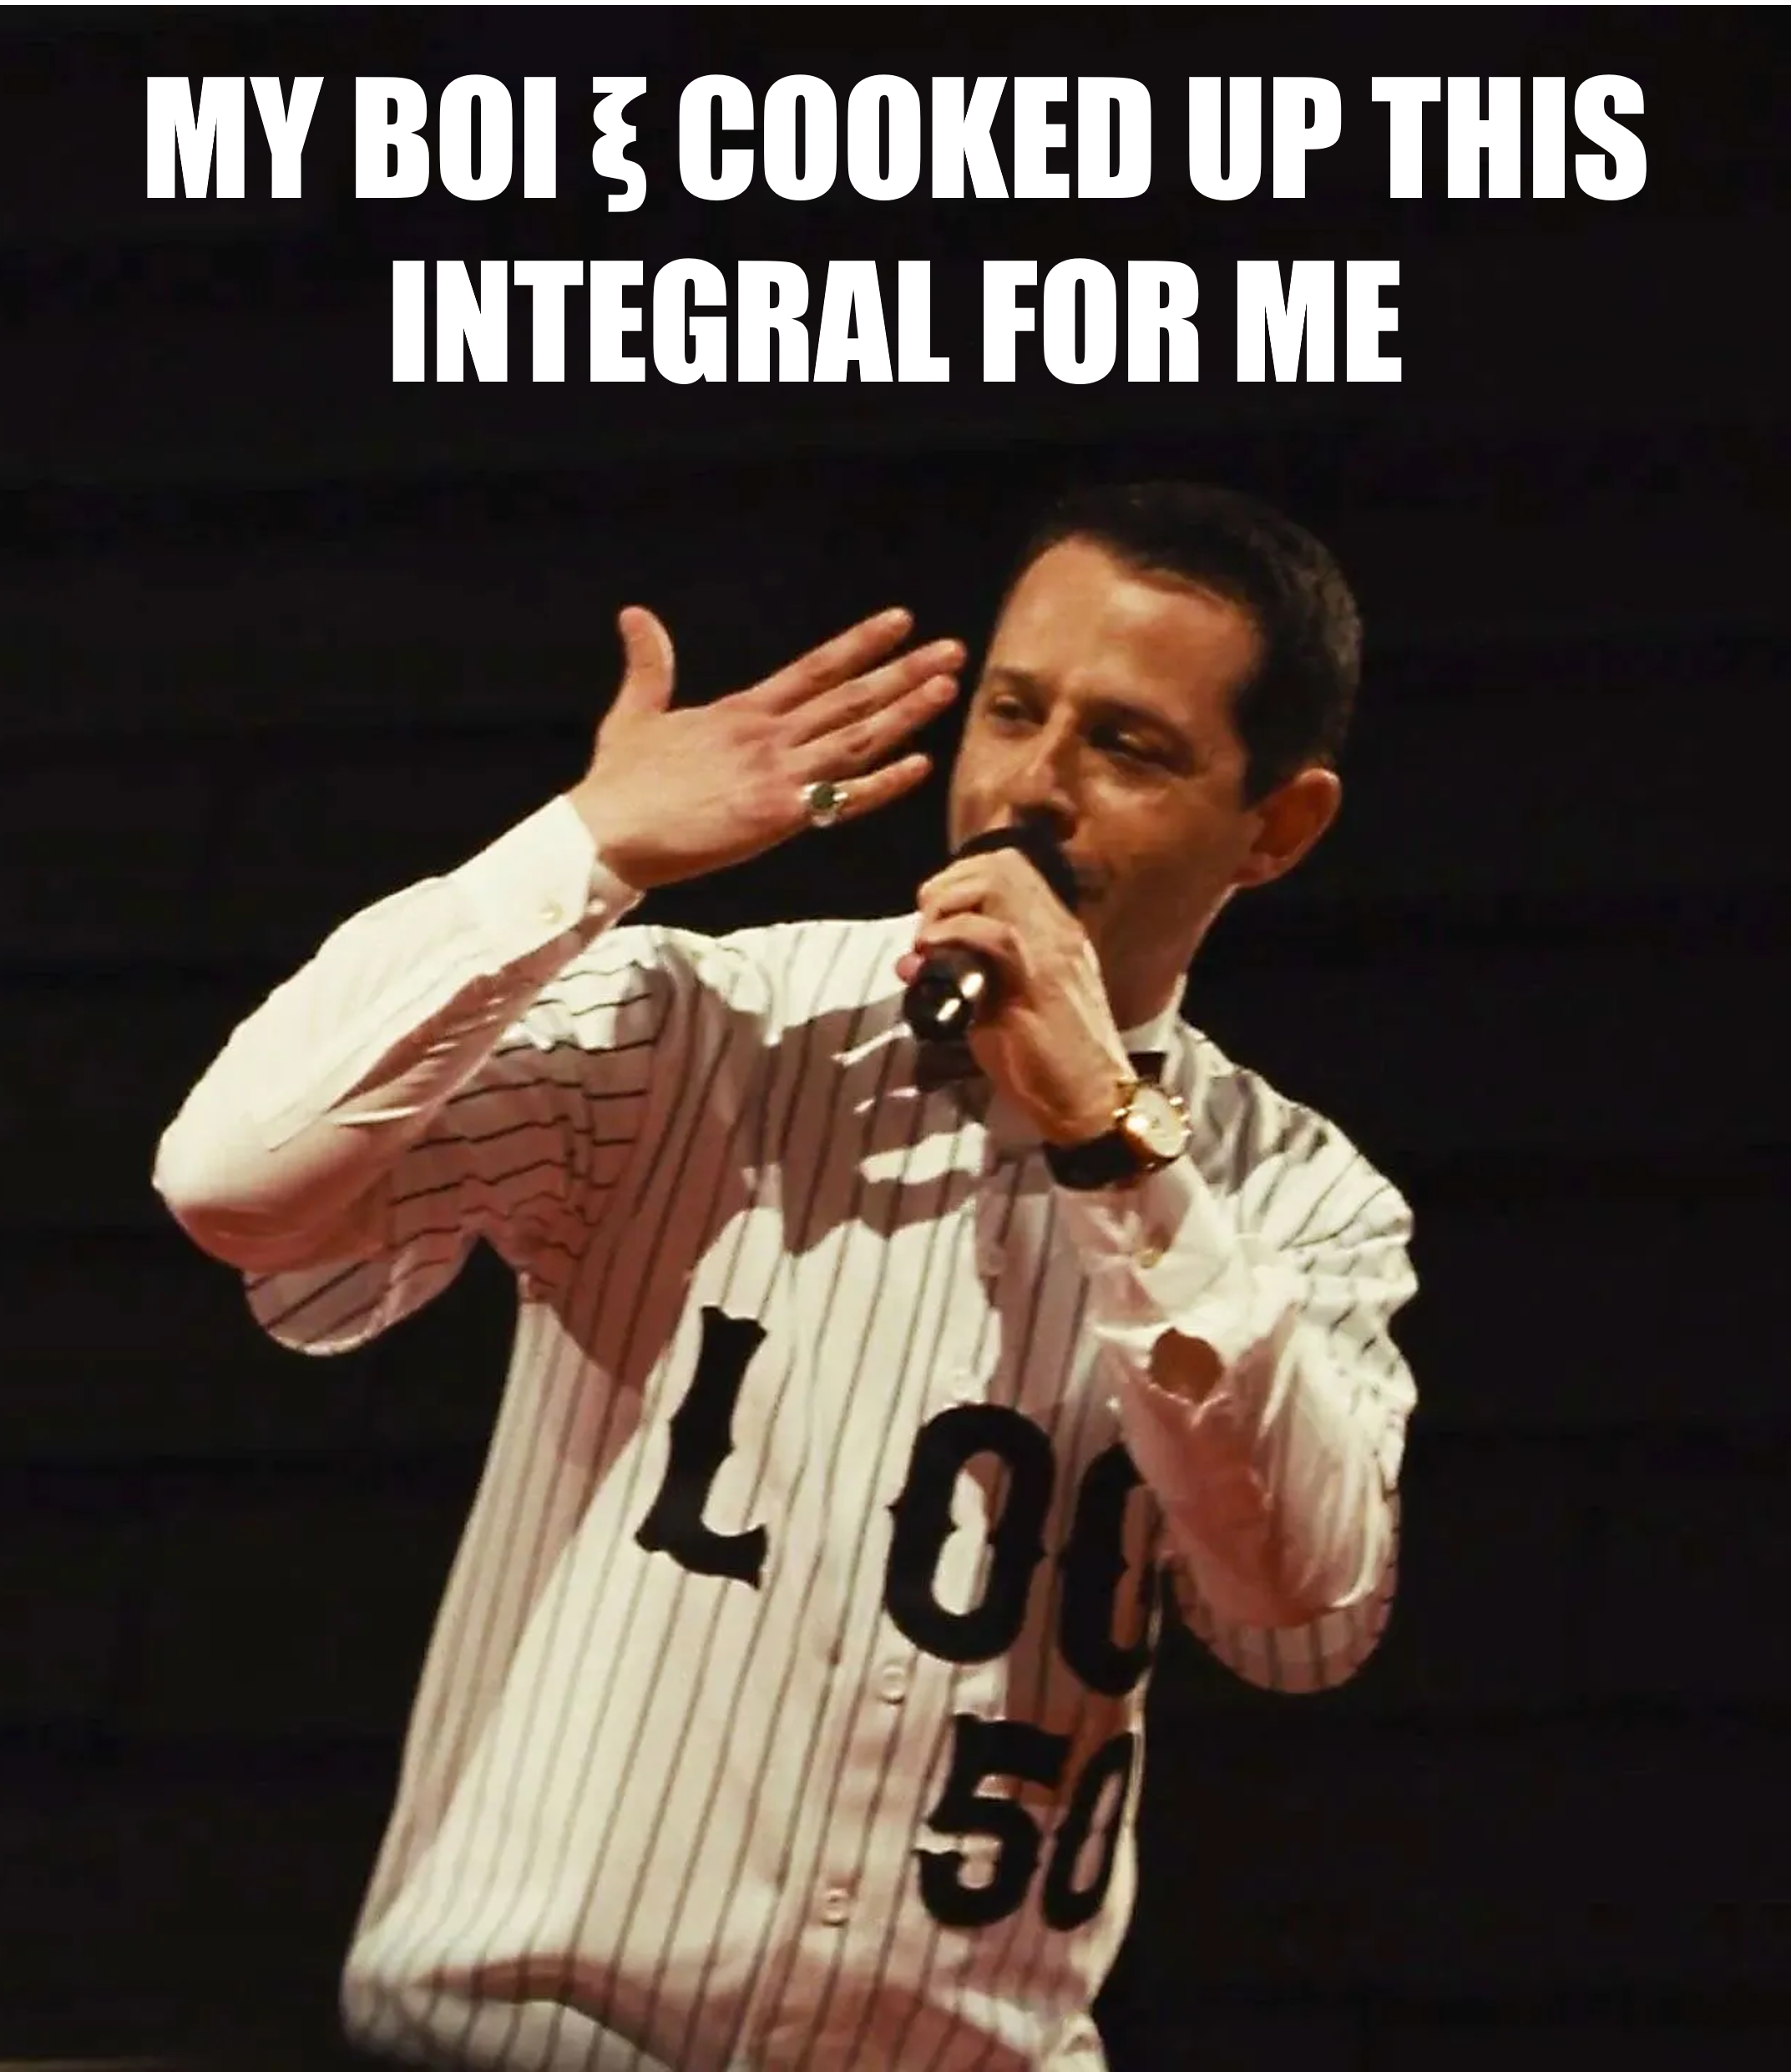
\includegraphics[width=3.375in]{corr_contour.png}
	\caption{Poles (black dots) and contour (blue line) used to evaluate \autoref{integraly} for (a) anti-correlated and (b) correlated modes.} 
	\label{fig:contours}
\end{figure}

\subsubsection{Anti-correlated Modes}
For anti-correlated modes, the poles are situated in the complex plane as shown in \autoref{fig:contours}a.
Since \autoref{integraly} is evaluated along the real axis, one can choose to evaluate the contour in the upper or lower half of the complex plane.
Since evaluating the residues in the upper or lower half of the complex plane yields the same result for \autoref{integraly}, we choose the contour which wraps around the least number of poles.

It is clear for c = -1 that there are four poles: $\pm i \sigma, \Delta_{ga}(0), \Delta_{ba}(0)$. 
Following \autoref{fig:contours}, the contour that wraps the upper half of the complex plane has only one pole, $i \sigma$; as such, we choose to evaluate \autoref{integraly} in the upper half of the complex plane for the case of anti-correlated modes through the residue theorem as
	\begin{equation}
		\begin{split}
			\rho_{ba} = \int_{-\infty}^\infty \mathrm{d}\xi P(\xi) \rho_{ba}(\xi) &= 2\pi i \sum_k \lim_{\xi \rightarrow \xi_k} P(\xi) \rho_{ba}(\xi) (\xi - \xi_k)\\
			&= 2\pi i \frac{\eta \sigma}{\pi} \lim_{\xi \rightarrow i\sigma} \frac{1}{(\xi + i\sigma)(\xi - i\sigma)} \frac{1}{\Delta_{ga}(0) - \xi} \frac{1}{\Delta_{ba}(0) - \xi} (\xi - i \sigma)\\
			&= 2\eta \sigma i \frac{1}{2i\sigma} \frac{1}{\Delta_{ga}(0) - i\sigma} \frac{1}{\Delta_{ba}(0) - i\sigma}\\
			&= \frac{\eta}{\Delta_{ga}(i\sigma)\Delta_{ba}(i \sigma)}\\
		\end{split}
	\end{equation}


In words, we see the inhomogeneous envelope width $\sigma$ is added to the linewidth of each resonance (e.g., $\Gamma_{ba} \rightarrow \Gamma_{ba} + \sigma$).
Therefore, pathway I-a cannot linenarrow anti-correlated modes. 
\subsubsection{Correlated Modes}
For correlated modes, the poles are situated in the complex plane as shown in \autoref{fig:contours}b.
It is clear that no matter which contour is chosen, there is a contribution to the final integral from either $\Delta_{ba}(0)$ or $\Delta_{ga}(0)$. 
For the below calculation, we choose to evaluate along the contour in the bottom half of the complex plane, i.e., the poles ($\xi_k$) are $-i\sigma, \Delta_{ga}$.
We stress that since the integral is evaluated over $\mathbb{R}$ and there are no degenerate poles, the results below can be obtained by evaluating the contour which wraps around the poles $i\sigma, \Delta_{ba}$ using the Residue theorem as 

	\begin{equation}
		\begin{split}
			\int_{-\infty}^\infty \mathrm{d}\xi P(\xi) \rho_{ba}(\xi) &= 2\pi i \sum_k \lim_{\xi \rightarrow \xi_k} P(\xi) \rho_{ba}(\xi) (\xi - \xi_k)\\
			&= 2\pi i \frac{\eta \sigma}{\pi} ( \lim_{\xi \rightarrow -i\sigma} \frac{1}{(\xi + i\sigma)(\xi - i\sigma)} \frac{1}{\Delta_{ga}(0) - \xi} \frac{1}{\Delta_{ba}(0) - \xi} (\xi + i \sigma) \\ &+
			\lim_{\xi \rightarrow \Delta_{ga}(0)} \frac{1}{(\xi + i\sigma)(\xi - i\sigma)} \frac{1}{\Delta_{ga}(0) - \xi} \frac{1}{\Delta_{ba}(0) - \xi} (\xi - \Delta_{ga}))\\
%			&= 2 \eta i \sigma (\frac{1}{2 i \sigma} \frac{1}{-i \sigma - \Delta_{ga}(0)} \frac{1}{\Delta_{ba}(0) - i\sigma} ) - 2 \eta i \sigma (\frac{1}{\sigma^2 + (\Delta_{ga} (0))^2} \frac{1}{\Delta_{ga}(0) + \Delta_{ba}(0)} )\\
			&= -\frac{\eta}{\Delta_{ga}(0) + i \sigma} (\frac{1}{\Delta_{ba}(0) - i \sigma} + \frac{2i\sigma}{(\Delta_{ga}(0) - i \sigma)(\Delta_{ga}(0) + \Delta_{ba}(0))})\\
		\end{split}
	\end{equation}
The final line of the above equation shows the presence of a new term, $\frac{2i\sigma}{\Delta_{ga}(0) + \Delta_{ba}(0)}$. 
This term is amplified by the width of the inhomogeneous envelope ($\sigma$) and has a linewidth $\Gamma_{ba} + \Gamma_{ga}$, which linenarrows the transition. 
Results for the other pathways follow the same technique.
\end{widetext}
%Generally, when starting from the ground state, non-parametric spectroscopies line-narrow correlated modes, and parametric spectroscopies line-narrow anti-correlated modes. \cite{Dick83_1, RN425}


\section{References}
% Create the reference section using BibTeX:
\bibliography{library.bib}

\end{document}
%
% ****** End of file apstemplate.tex ******

